\chapter{Bewertungsschema}

Nach dem Einbinden der MNIST Daten und dem Erstellen des Models mitsamt allen benötigten Placeholdern und Variablen ist es nun an der Zeit festzustellen, wie nahe die Prädiktionen des Models an der Realität sind. Dafür wird in diesem Workshop eine mathematische Methode namens Cross-Entropy verwendet. In kürzester und einfachster Form beschrieben, liefert Cross-Entropy einen Zahlenwert, welcher die Distanz zwischen dem One-Hot Vektor des Labels mit jenem der Prädiktion liefert. Diese Distanz wird Loss genannt und beschreibt den Fehler des Models bei der Prädiktion. Die Formel von Cross-Entropy lautet dabei: $ - \sum{y' * \ln{y}}$. 

Cross-Entropy
\begin{figure}[!ht]
\centering
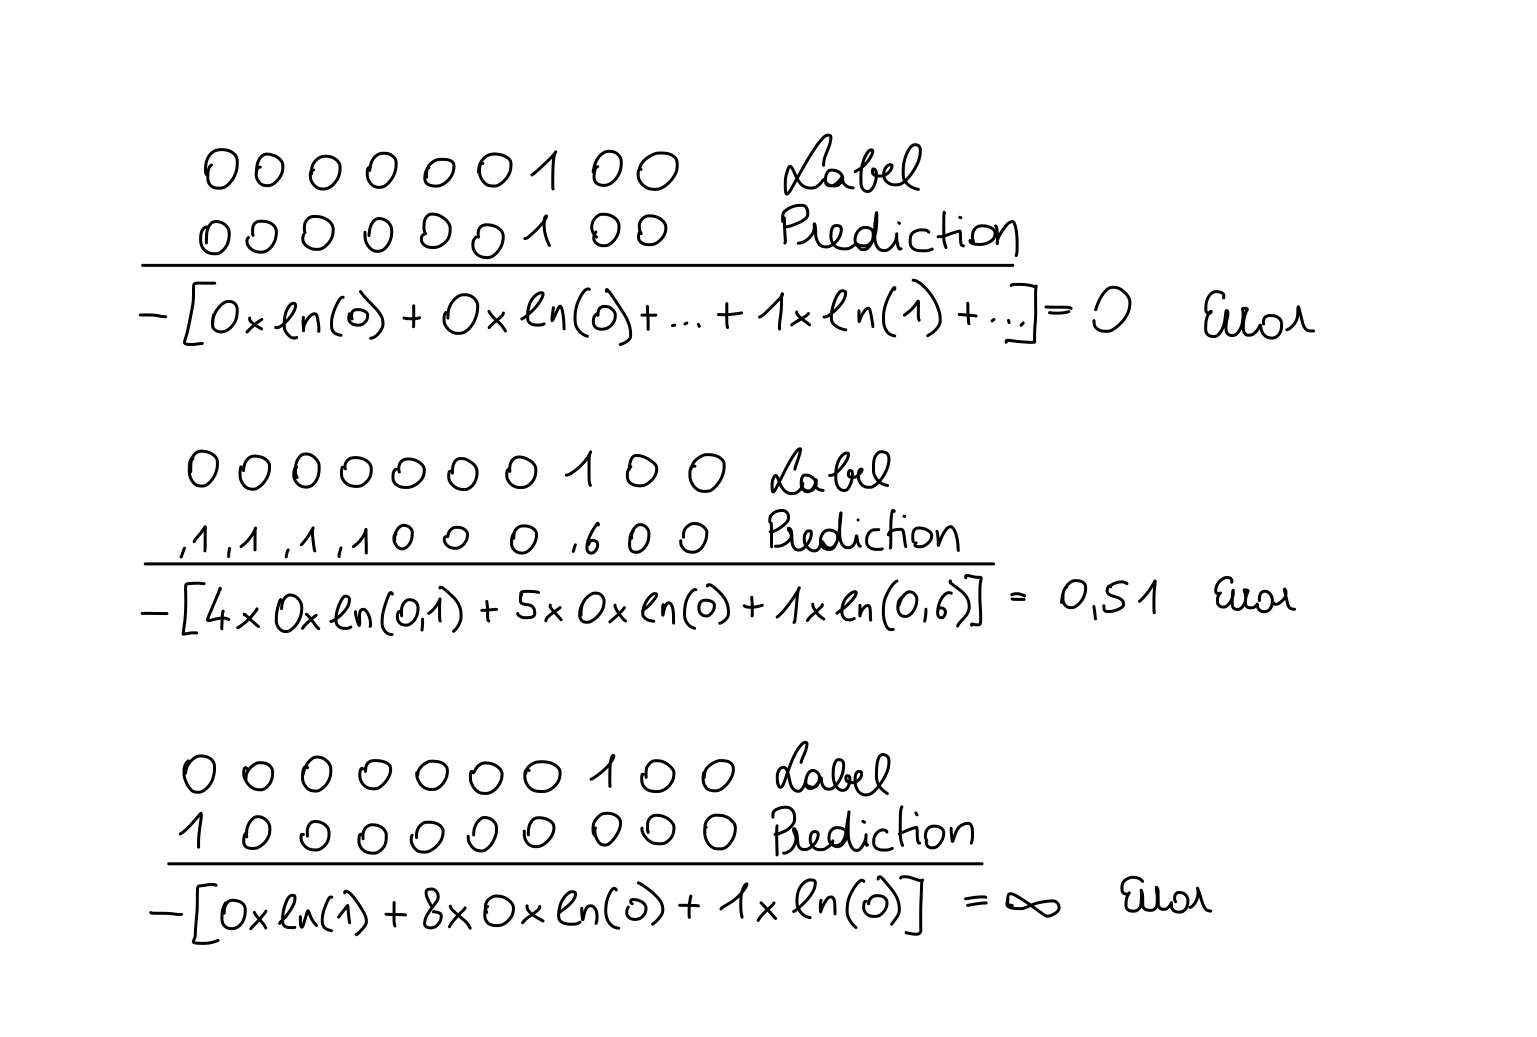
\includegraphics[width=1.00\textwidth]{images/crossEntropy}
\caption{Cross-Entropy Beispiel}
\label{fig:cross_entropy}
\end{figure}

Nun, da ein passendes Bewertungsschema gefunden wurde, ist es an der Zeit, dieses in den Code zu integrieren. Gleich wie beim Model, macht es wiederum Sinn, dieser Funktion einen eigenen \textbf{\textit{name\_scope}} zu geben.

\lstset{language=Python}
\definecolor{listinggray}{gray}{0.95} 
\definecolor{keyword}{rgb}{0.4, 0, 0.1} 
\definecolor{comment}{rgb}{0, 0.4, 0}
% Zuweisen der Farben zu den entsprechenden Elementen ... 
\lstset{keywordstyle=\color{keyword}\bfseries} 
\lstset{commentstyle=\color{comment}} 
\lstset{backgroundcolor=\color{listinggray}}


\begin{lstlisting}
with tf.name_scope('Loss'):
	cost = tf.reduce_mean(-tf.reduce_sum(y*tf.log(pred)))
\end{lstlisting}


	
	
Betrachtet man die zweite Zeile genauer, scheint es eventuell erstmals nicht ganz klar, was hier berechnet wird. Dies ist allerdings schnell geklärt. Der Teil innerhalb von \textbf{\textit{tf.reduce\_mean}} beinhaltet lediglich die mathematische Formel von Cross-Entropy $ - \sum{y' * \ln{y}}$. Da wir allerdings beim Model (pred) möglicherweise nicht nur ein einzelnes Bild evaluieren lassen möchten (die Anzahl der Bilder in InputData ist nicht begrenzt), wird über \textbf{\textit{tf.reduce\_mean}} der Mittelwert über alle Einzelfehler aller zu evaluierenden Bilder berechnet.


\label{cha:Bewertungsschema}